\documentclass{article}
\usepackage[%
  left=1.5cm, right=1.5cm, top=1.5cm, bottom=2.0cm%
]{geometry}
\usepackage{multicol}
\usepackage{booktabs}
\usepackage{ragged2e}
\usepackage{array}
\usepackage{tikz}
\usetikzlibrary{calc}
\usepackage{amsmath}
\usepackage{amssymb}

\title{Kinematics Concept Map and Relationships}
\author{TCB}

\begin{document}
\maketitle

\begin{center}
%\usepackage{tikz}
%\usetikzlibrary{calc}
%\usepackage{amsmath}

%\usepackage{tikz}
%\usetikzlibrary{calc}
%\usepackage{amsmath}


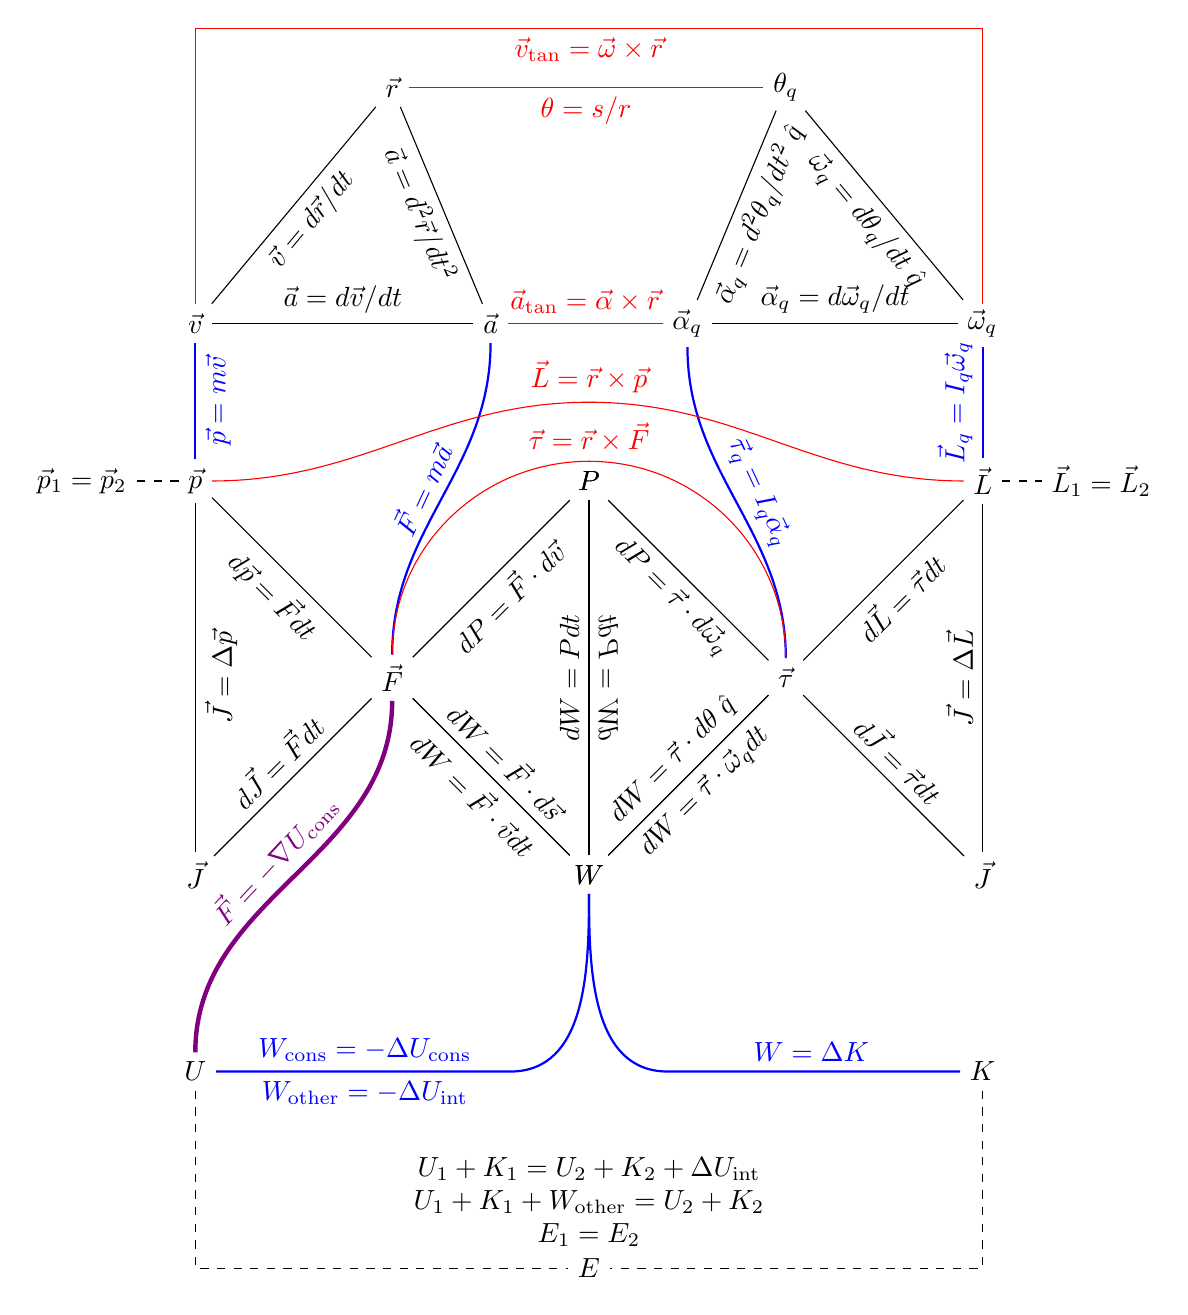
\begin{tikzpicture}
  \def\baseSep{2.5}
  % Energy section: nodes
  \node (E) at (2*\baseSep, 0) {$E$};
  \node (U) at ($(E)+(-2*\baseSep,\baseSep)$) {$U$};
  \node (K) at ($(E)+(2*\baseSep,\baseSep)$) {$K$};

  % Force section: nodes
  \node (vF) at ($(E)+(-1*\baseSep, 3*\baseSep)$) {$\vec{F}$};
  \node (vJ) at ($(vF)+(-\baseSep, -\baseSep)$) {$\vec{J}$};
  \node (W) at ($(vF)+(\baseSep, -\baseSep)$) {$W$};
  \node (vp) at ($(vF)+(-\baseSep, \baseSep)$) {$\vec{p}$};
  \node (P) at ($(vF)+(\baseSep, \baseSep)$) {$P$};
  \draw [dashed] (vp) -- ++(-0.3*\baseSep,0) node [left] {$\vec{p}_1=\vec{p}_2$};

  % Descriptor section: nodes
  \node (vr) at ($(vF)+(0,3*\baseSep)$) {$\vec{r}$};
  \node (vv) at ($(vr)+(-\baseSep, -1.2*\baseSep)$) {$\vec{v}$};
  \node (va) at ($(vr)+(0.5*\baseSep, -1.2*\baseSep)$) {$\vec{a}$};


  % Descriptor section: connections
  \draw (vv) -- (vr) node [midway, below, sloped] %
  {$\vec{v}=d\vec{r}/dt$};
  \draw (vr) -- (va) node [midway, below, sloped] %
  {$\vec{a}=d^2\vec{r}/dt^2$}; 
  \draw (vv) -- (va) node [midway, above, sloped] %
  {$\vec{a}=d\vec{v}/dt$}; 

  % Force section: connections
  \draw (vp) -- (vF) node [midway, below, sloped] %
  {$d\vec{p}=\vec{F}dt$};
  \draw (vF) -- (P) node [midway, below, sloped] %
  {$dP=\vec{F}\cdot d\vec{v}$};
  \draw (vF) -- (W) node [midway, above, sloped] %
  {$dW=\vec{F}\cdot d\vec{s}$};
  \draw (vF) -- (W) node [midway, below, sloped] %
  {$dW=\vec{F}\cdot \vec{v}dt$};
  \draw (vJ) -- (vF) node [midway, above, sloped] %
  {$d\vec{J}=\vec{F}dt$};
  \draw (vJ) -- (vp) node [midway, below, sloped] %
  {$\vec{J}=\Delta\vec{p}$};
  \draw (W) -- (P) node [midway, above, sloped] %
  {$dW=P dt$};

  % Energy section: connections
  \draw [dashed] (U) |- (E);
  \draw [dashed] (K) |- (E);
  \node (consE-abstract) at ($(E)+(0,\baselineskip)$) %
  {$E_1=E_2$};
  \node (consE-Wother) at ($(E)+(0,2*\baselineskip)$) %
  {$U_1+K_1+W_{\text{other}}=U_2+K_2$};
  \node (consE-Uint) at ($(E)+(0,3*\baselineskip)$) %
  {$U_1+K_1=U_2+K_2+\Delta U_{\text{int}}$};

  % Inter section: connections
  % Work and energy
  \node (joinW) at ($(E)+(0,\baseSep)$) {};
  \draw [thick, blue] (W) to [out=-90, in=0] ($(joinW)+(-0.4*\baseSep, 0)$) -- (U) ;
  \draw [thick, blue] (W) to [out=-90, in=180] ($(joinW)+(0.4*\baseSep, 0)$) -- (K) ;
  \path (U) -- (K) node [blue, pos=0.2, above] {$W_{\text{cons}}=-\Delta U_{\text{cons}}$};
  \path (U) -- (K) node [blue, pos=0.2, below] {$W_{\text{other}}=-\Delta U_{\text{int}}$};
  \path (U) -- (K) node [blue, pos=0.8, above]  {$W=\Delta K$};
  % Energy and force
  \draw [ultra thick, blue!50!red] (U) to[out=90, in=-90] (vF);
  \path (U) -- (vF) node [midway, above, rotate=47, blue!50!red] % 
  {$\vec{F} = -\nabla U_{\text{cons}}$};
  % Force and descriptors
  \draw [thick, blue] (vF) to[out=90, in=-90] (va);
  \path (vF) -- (va) node [midway, above, rotate=65, blue] %
  {$\vec{F}=m\vec{a}$};
  \draw [thick, blue] (vp) -- (vv) node [midway, below, sloped, blue] %
  {$\vec{p}=m\vec{v}$};


  %%%%%%%%%%%%%%%%%%%%%%%%%%%%%%%%%%%%%%%%%%%%%%%%%%
  %% Rotation

  
  % Torque section: nodes
  \node (vtau) at ($(E)+(1*\baseSep, 3*\baseSep)$) {$\vec{\tau}$};
  \node (vJang) at ($(vtau)+(\baseSep, -\baseSep)$) {$\vec{J}$};
  \node (Wang) at ($(vtau)+(-\baseSep, -\baseSep)$) {$W$};
  \node (vL) at ($(vtau)+(\baseSep, \baseSep)$) {$\vec{L}$};
  \node (Pang) at ($(vtau)+(-\baseSep, \baseSep)$) {$P$};

  % Descriptor section: nodes
  \node (theta) at ($(vtau)+(0,3*\baseSep)$) {$\theta_q$};
  \node (vomega) at ($(theta)+(\baseSep, -1.2*\baseSep)$) {$\vec{\omega}_q$};
  \node (valpha) at ($(theta)+(-0.5*\baseSep, -1.2*\baseSep)$) {$\vec{\alpha}_q$};


  % Descriptor section: connections
  \draw (vomega) -- (theta) node [midway, below, sloped] %
  {$\vec{\omega}_q=d\theta_q/dt \;\hat{q}$};
  \draw (theta) -- (valpha) node [midway, below, sloped] %
  {$\vec{\alpha}_q=d^2\theta_q/dt^2 \;\hat{q}$}; 
  \draw (vomega) -- (valpha) node [midway, above, sloped] %
  {$\vec{\alpha}_q=d\vec{\omega}_q/dt$}; 

  % Torque section: connections
  \draw (vL) -- (vtau) node [midway, below, sloped] %
  {$d\vec{L}=\vec{\tau}dt$};
  \draw (vtau) -- (Pang) node [midway, below, sloped] %
  {$dP=\vec{\tau}\cdot d\vec{\omega}_q$};
  \draw (vtau) -- (Wang) node [midway, above, sloped] %
  {$dW=\vec{\tau}\cdot d\theta \;\hat{q}$};
  \draw (vtau) -- (Wang) node [midway, below, sloped] %
  {$dW=\vec{\tau}\cdot \vec{\omega}_qdt$};
  \draw (vJang) -- (vtau) node [midway, above, sloped] %
  {$d\vec{J}=\vec{\tau}dt$};
  \draw (vJang) -- (vL) node [midway, above, sloped] %
  {$\vec{J}=\Delta\vec{L}$};
  \draw (Wang) -- (Pang) node [midway, below, sloped] %
  {\raisebox{\depth}{\scalebox{1}[-1]{$dW=P dt$}}};
  \draw [dashed] (vL) -- ++(0.3*\baseSep,0) node [right] {$\vec{L}_1=\vec{L}_2$};

  % Inter section: connections
  % Torque and descriptors
  \draw [thick, blue] (vtau) to[out=90, in=-90] (valpha);
  \path (valpha) -- (vtau) node [midway, above, rotate=-65, blue] %
  {$\vec{\tau}_q=I_q\vec{\alpha}_q$};
  \draw [thick, blue] (vL) -- (vomega) node [midway, above, sloped, blue] %
  {$\vec{L}_q=I_q\vec{\omega}_q$};



  %%%%%%%%%%%%%%%%%%%%%%%%%%%%%%%%%%%%%%%%%%%%%%%%%%
  % Inter kinematic connections
  \draw [red] (vF) to [out=90, in=180] ($(P)+(0,0.1*\baseSep)$) to
  [out=0, in=90] (vtau); %
  \node [red, above] (tauEQrxF) at ($(P)+(0,0.1*\baseSep)$) {$\vec{\tau}
    = \vec{r} \times \vec{F}$}; %
  \draw [red] (va) -- (valpha) node [midway, above]
  {$\vec{a}_{\text{tan}}=\vec{\alpha} \times \vec{r}$};
  \draw [red] (vr) -- (theta) node [midway, below] {$\theta = s / r$};
  \draw [red] (vv) -- ++(0,1.5*\baseSep) -- ++(4*\baseSep, 0) node
  [midway, below] {$\vec{v}_{\text{tan}} = \vec{\omega} \times \vec{r}$} --
  ++(0,-1.4*\baseSep);
  \coordinate (joinMomenta) at ($(P)+(0,0.4*\baseSep)$);
  \draw [red] (vp) to [out=0, in=180] (joinMomenta) to [out=0, in=180]
  (vL);
  \node [red, above] (momRelate) at (joinMomenta) {$\vec{L} = \vec{r}
    \times \vec{p}$}; 

\end{tikzpicture}


\end{center}
Main concepts in translational (left hand) and rotational (right hand)
motion are nodes in the network.  The concepts are collected by category as
descriptors (top), dynamics (middle), and energy (bottom). Work, energy,
and power are common between translational and rotational motion.
Connections between concepts are edges that are labeled with their
mathematical relationships. Those in blue represent inter-category
relations within each type of motion and those in red represent connections
between linear and angular motion.  The purple edge is the special relation
between force and potential energy. Dashed edges indicate conservation
laws. 



\newpage
\begin{multicols}{2}

  \begin{tabular}{>{$}l<{$}>{\RaggedRight}p{0.2\linewidth}>{$}l<{$}>{\RaggedRight}p{0.4\linewidth}}
    \toprule
    \multicolumn{2}{c}{\bfseries Linear}
    &\multicolumn{2}{c}{\bfseries Angular}%
    \\
    \multicolumn{2}{c}{\bfseries  (Translational)}
    &\multicolumn{2}{c}{\bfseries (Rotational)}%
    \\

    \midrule
    t & time & t & time\\
    \vec{r} & position & \theta_q & angular position around axis $q$\\
    \vec{v} & velocity & \vec{\omega}_q &  angular velocity around axis $q$\\
    \vec{a} & acceleration & \vec{\alpha}_q &  angular acceleration around axis $q$\\
    \midrule
    m & mass & I_q & moment of inertia about axis $q$\\
    \vec{p} & momentum & \vec{L} & angular momentum\\
    \vec{F} & force & \vec{\tau} & torque \\
    %\midrule
    %K_{\text{lin}} & $\frac{1}{2}mv^2$ & K_{\text{ang}} & $=\frac{1}{2}I\omega^2$\\
    \bottomrule
  \end{tabular}
  
  \begin{tabular}{>{$}l<{$}>{\RaggedRight}p{0.8\linewidth}}
    \toprule
    P & power\\
    \vec{J} & impulse\\
    W & work\\
    \midrule %
    U & potential energy\\
    K & kinetic energy\\
    U_{\text{cons}} & potential due to conservative interactions\\
    W_{\text{cons}} & work done by conservative interactions\\
    U_{\text{int}} & internal energy\\
    W_{\text{other}} & work done by interactions not accounted for explicitly\\
    E & total energy\\
    \midrule %
    q & generic variable for discussion of operations\\
    \Delta q & difference between final and initial values of $q$ ($\Delta q
    \equiv q_{\text{final}} - q_{\text{initial}}$)\\
    dq & differential element $q$\\
    \hat{n} & unit normal vector to the plane defined by $q_1$ and $q_2$;
    direction defined by right-hand rule\\
    \vec{q}_1\cdot\vec{q}_2 & scalar (dot) product between $q_1$ and $q_2$
    ($\vec{q}_1\cdot\vec{q}_2 = |\vec{q}_1||\vec{q}_2|\cos(\phi_{1,2})$)\\
    \vec{q}_1 \times \vec{q}_2 & vector product between $q_1$ and $q_2$
    ($\vec{q}_1\times\vec{q}_2 = |\vec{q}_1||\vec{q}_2|\sin(\phi_{1,2})\;\hat{n}$)\\
    \bottomrule
  \end{tabular}
  
\end{multicols}




\end{document}
